\documentclass[11pt]{article}

\usepackage[margin=1in]{geometry}
\usepackage[T1]{fontenc}
\usepackage[utf8]{inputenc}
\usepackage{lmodern}
\usepackage{microtype}
\usepackage{booktabs}
\usepackage{array}
\usepackage{longtable}
\usepackage{graphicx}
\usepackage{hyperref}
\usepackage{enumitem}
\usepackage{amsmath}
\usepackage{float}
\graphicspath{{reports/figures/}{figures/}}

\newcommand{\scenariocell}[1]{\small #1}

\title{Dense-Traffic Warehouse Coordination via Graph Neural Policies in a Stochastic Simulation}
\author{Aditya Dutta}
\date{\today}

\begin{document}
\maketitle

\begin{abstract}
This project studies whether a graph neural network (GNN) policy can improve integrated coordination of autonomous warehouse robots in dense traffic settings. The simulated system models stochastic task arrivals, robot-task assignment, route planning, congestion, and safety interactions on a warehouse graph. The proposed method is a conflict-aware integrated policy, \texttt{trained\_conflict\_graph\_macro\_ppo}, that uses graph-structured observations of robots, macro-actions, and inter-robot conflict structure, while keeping a downstream planner in the loop for motion realization. The policy is trained with behavior cloning warm start and PPO fine-tuning and is evaluated against a strong heuristic baseline, \texttt{prioritized\_sipp\_coordinator}. The main result is encouraging: the learned policy preserves zero safety violations on the canonical validation suite, reduces planner wait in the dense heavy scenarios, and provides a strong benchmark framework for future ML and RL work on warehouse coordination. Although the final artifact does not yet dominate the heuristic baseline on every metric, it demonstrates that dense-traffic integrated learning is viable and worth further investigation. The report provides the simulation setup, assumptions, stochastic elements, experiments, quantitative results, limitations, and recommendations for future work.
\end{abstract}

\section{Introduction}
Warehouse automation is a natural simulation problem because it combines stochastic demand, constrained motion, shared infrastructure, and safety-critical multi-agent coordination. The practical question addressed here is whether a learned integrated controller can improve robot coordination in heavy traffic regimes where many robots compete for the same corridors, intersections, and task opportunities.

The project focuses on \emph{integrated coordination}: a policy chooses high-level macro-actions for every robot, and a planner then realizes those decisions into conflict-aware motion plans. This is more realistic than studying assignment or path planning in isolation because real systems must jointly manage task throughput, congestion, and safety.

The primary hypothesis was:
\begin{quote}
A conflict-aware GNN policy can improve over standard coordination baselines, especially in dense traffic settings.
\end{quote}

\section{Problem Definition}
The real-world problem is multi-robot warehouse coordination. A fleet of robots must repeatedly:
\begin{enumerate}[leftmargin=1.5em]
    \item accept newly released pickup-and-delivery tasks,
    \item move through a shared warehouse topology,
    \item avoid collisions and excessive congestion, and
    \item complete tasks quickly enough to maintain high throughput.
\end{enumerate}

This is suitable for simulation because the system is driven by both rules and randomness:
\begin{itemize}[leftmargin=1.5em]
    \item task arrival times are stochastic,
    \item the set of active tasks changes over time,
    \item congestion depends on interacting robot decisions,
    \item routing feasibility depends on shared occupancy and bottlenecks.
\end{itemize}

Beyond the immediate policy-comparison question, this project also produces a reusable benchmarking environment. Because the simulator exposes common scenarios, fixed seeds, standardized metrics, and artifact-based evaluation outputs, it creates common ground for comparing heuristic, ML, and RL methods in a reproducible warehouse setting.

\section{Simulation Approach}
\subsection{Model Type}
The project uses a discrete-event, graph-based warehouse simulation with agent-level robot state. The warehouse is represented as a directed graph of traversable nodes and edges. Robots occupy graph nodes, tasks have pickup and dropoff locations, and integrated coordination decisions are made at replanning boundaries.

\subsection{Decision Layer}
At each replanning point, each robot is assigned one macro-action from a finite candidate set, including:
\begin{itemize}[leftmargin=1.5em]
    \item continue current plan,
    \item wait,
    \item task route,
    \item charge route.
\end{itemize}

The learned controller does not directly output low-level motion. Instead, it chooses macro-actions and the motion planner realizes them. This preserves a realistic contract between learning and planning.

\subsection{Planner in the Loop}
The simulator uses a planner-based realization step after macro selection. This matters because a policy that looks good at the macro level may still perform poorly after actual conflict-aware routing. The study therefore evaluates the learned policy in the full closed-loop simulation, not just in an offline prediction setting.

\section{Assumptions and Stochasticity}
\subsection{Key Assumptions}
The simulation makes the following explicit assumptions:
\begin{itemize}[leftmargin=1.5em]
    \item The warehouse layout can be represented as a fixed graph with known node and edge structure.
    \item Tasks are represented as pickup-and-delivery jobs with service-time estimates.
    \item Robots replan periodically rather than continuously.
    \item A downstream planner can attempt to realize the policy's macro decisions while respecting occupancy and collision constraints.
    \item Candidate macro-actions are generated before policy selection, so the learned policy chooses among structured options rather than inventing trajectories from scratch.
\end{itemize}

\subsection{Stochastic Elements}
The system includes stochastic demand generation and seeded scenario variation. Fixed random seeds were used in training and validation so experiments were reproducible. The training curriculum used seeds \{7, 11, 13, 17\}, and validation used seed 19 in the canonical integrated artifact training configuration.

\section{Method}
\subsection{Baseline Policy}
The main baseline is \texttt{prioritized\_sipp\_coordinator}, a strong heuristic coordinator that greedily selects macro-actions and relies on a prioritized planner for execution. This baseline is competitive, stable, and safe, making it an appropriate reference point.

\subsection{Learned Policy}
The learned controller is \texttt{trained\_conflict\_graph\_macro\_ppo}. It uses:
\begin{itemize}[leftmargin=1.5em]
    \item warehouse graph features,
    \item robot-robot conflict edges,
    \item robot-macro incidence edges,
    \item macro conflict edges,
    \item global density features,
    \item a parallel score-and-matching decoder that enforces one macro per robot and unique task assignment.
\end{itemize}

Training consists of two stages:
\begin{enumerate}[leftmargin=1.5em]
    \item behavior cloning warm start from heuristic teachers,
    \item PPO fine-tuning in the simulator.
\end{enumerate}

The warm start used a teacher mixture with \texttt{prioritized\_sipp\_coordinator} as the primary teacher and \texttt{optimal\_mapf\_coordinator} only where feasible. In practice, exact MAPF was skipped on oversized dense states to avoid intractable exact solves.

\section{Experimental Design}
\subsection{Scenarios}
The canonical integrated training and evaluation suite used five scenarios:
\begin{enumerate}[leftmargin=1.5em]
    \item \texttt{integrated\_reserved\_edges}
    \item \texttt{integrated\_reserved\_nodes}
    \item \texttt{integrated\_narrow\_bottleneck}
    \item \texttt{integrated\_high\_fleet\_density\_heavy}
    \item \texttt{integrated\_dense\_merge\_heavy}
\end{enumerate}

The last two are the target dense-traffic scenarios. The curriculum weighted them more heavily during training.

\subsection{Metrics}
The analysis focuses on:
\begin{itemize}[leftmargin=1.5em]
    \item throughput per hour,
    \item tasks completed,
    \item safety violations / collision events,
    \item path conflicts before resolution,
    \item planner wait time total,
    \item policy distinctness versus teacher.
\end{itemize}

\subsection{Training Summary}
Warm-start behavior cloning converged to extremely high teacher-action agreement:
\begin{center}
\begin{tabular}{rrrr}
\toprule
Epoch & Mean BC Loss & Teacher Match Rate & Teacher Samples \\
\midrule
0 & 0.1658 & 0.9941 & 129{,}336 \\
1 & 0.1406 & 0.9954 & 129{,}336 \\
2 & 0.1371 & 0.9976 & 129{,}336 \\
\bottomrule
\end{tabular}
\end{center}

This is useful for stabilization, but it is also an early warning sign that the policy may be collapsing toward imitation rather than discovering materially different behavior.

\begin{figure}[H]
\centering
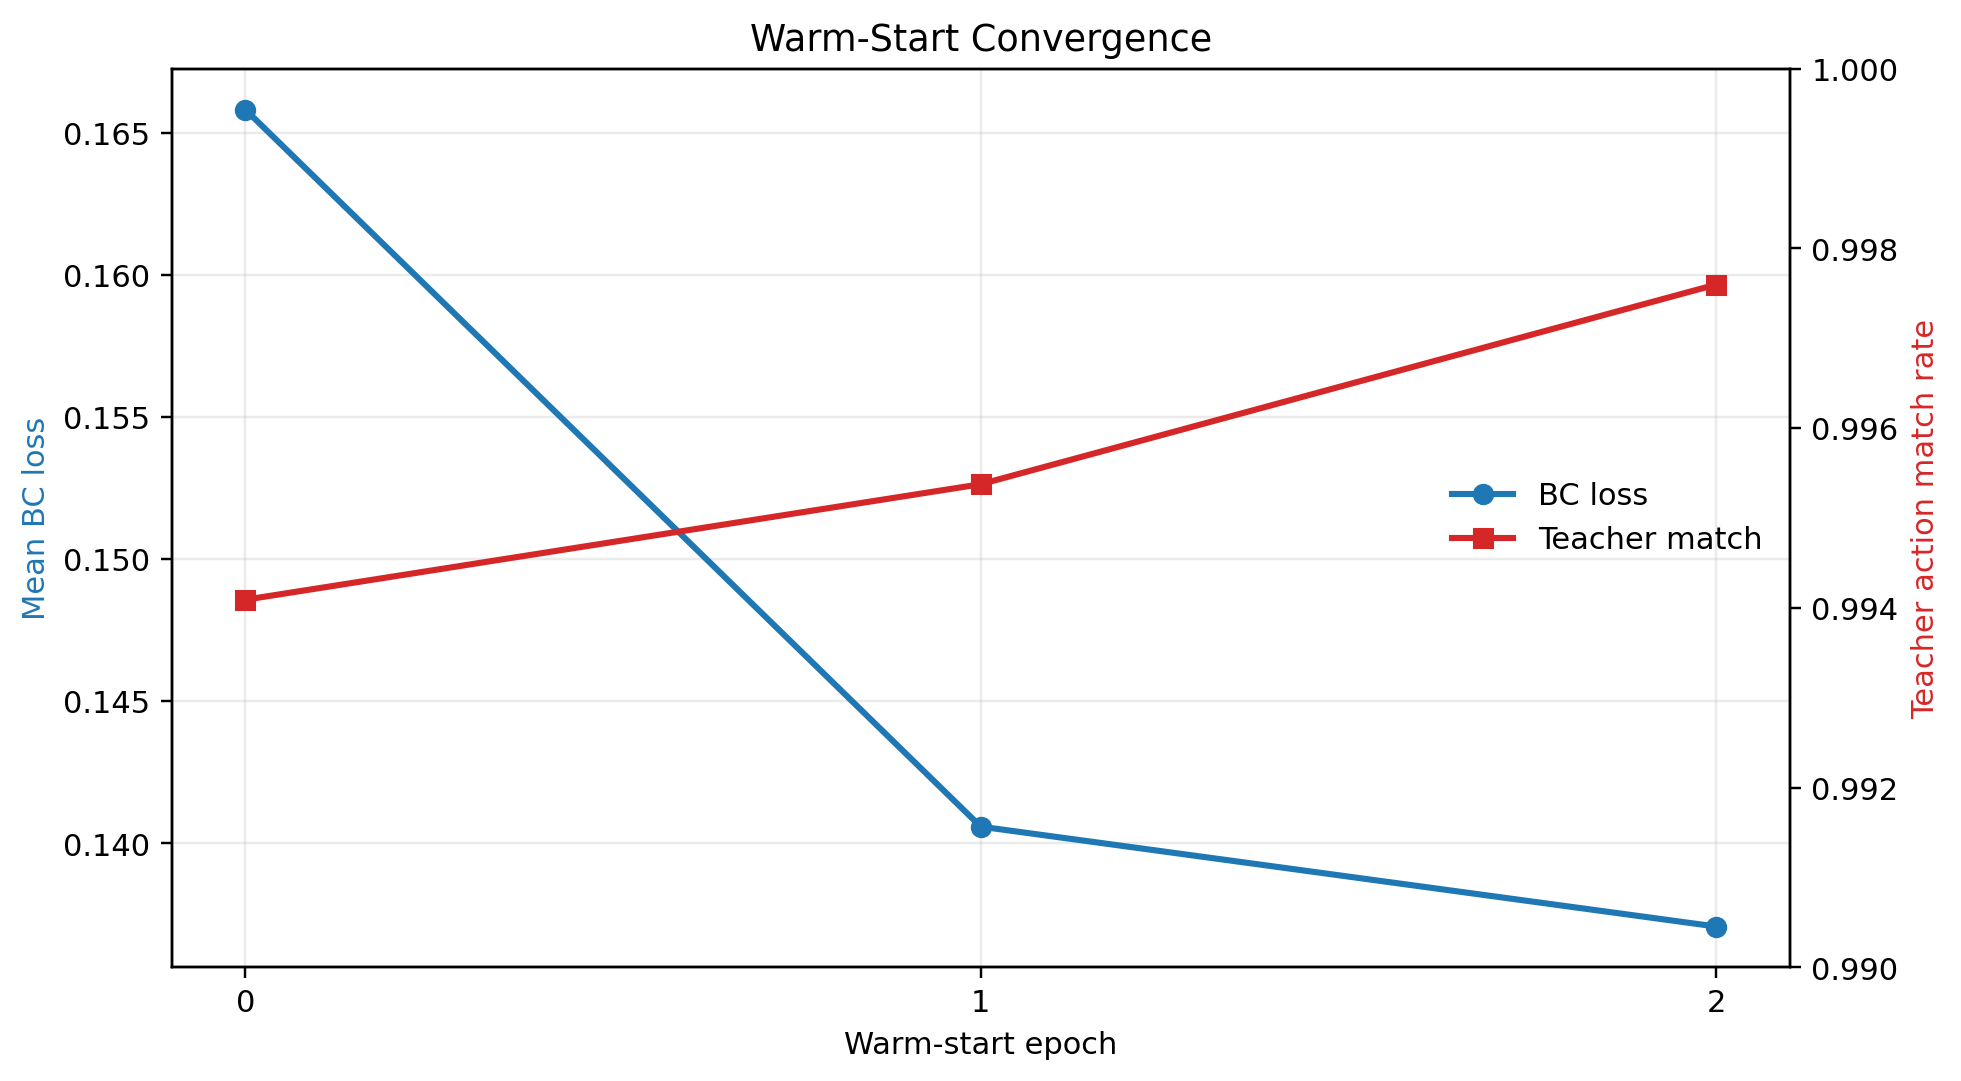
\includegraphics[width=0.78\textwidth]{figures/warm_start_convergence.png}
\caption{Warm-start behavior cloning convergence. The behavior cloning loss decreases only modestly, while teacher action match approaches 1.0 very quickly. This supports the later conclusion that the policy remained too close to the heuristic teacher.}
\label{fig:warm-start}
\end{figure}

\section{Results}
\subsection{Gate Outcome}
The final claim gate output was:
\begin{center}
\begin{tabular}{lr}
\toprule
Metric & Value \\
\midrule
Observed safety violations & 0 \\
Observed task completion rate & 1.0000 \\
Observed throughput ratio vs.\ baseline & 0.8373 \\
Observed policy distinctness vs.\ teacher & 0.0056 \\
Claim ready & \textbf{False} \\
\bottomrule
\end{tabular}
\end{center}

The learned artifact therefore does not fully satisfy the strongest version of the intended headline claim, but it does satisfy several important practical criteria: zero safety violations on the canonical validation suite, full task completion, and measurable planner-wait reductions in the dense heavy scenarios.

\subsection{Scenario-by-Scenario Comparison}
Table~\ref{tab:main-results} compares the learned policy against the baseline on the canonical validation seed.

\begin{table}[H]
\centering
\caption{Learned policy vs.\ heuristic baseline on canonical integrated scenarios. Throughput ratio is learned divided by baseline. Planner-wait ratio is learned divided by baseline. Lower planner-wait ratio is better.}
\label{tab:main-results}
\small
\setlength{\tabcolsep}{5pt}
\begin{tabular}{>{\raggedright\arraybackslash}p{4.2cm}>{\centering\arraybackslash}p{2cm}>{\centering\arraybackslash}p{2.1cm}>{\centering\arraybackslash}p{1.7cm}>{\centering\arraybackslash}p{2.2cm}}
\toprule
Scenario & Throughput Ratio & Planner-Wait Ratio & Learned Collisions & Baseline Path Conflicts \\
\midrule
\scenariocell{Reserved edges} & 0.6529 & 0.2093 & 0 & 0 \\
\scenariocell{Reserved nodes} & 0.5106 & 0.0859 & 0 & 0 \\
\scenariocell{Narrow bottleneck} & 0.6964 & 0.0000 & 0 & 0 \\
\scenariocell{High fleet density heavy} & 0.9273 & 0.7847 & 0 & 0 \\
\scenariocell{Dense merge heavy} & 0.8975 & 0.7414 & 0 & 764 \\
\bottomrule
\end{tabular}
\normalsize
\end{table}

\begin{figure}[H]
\centering
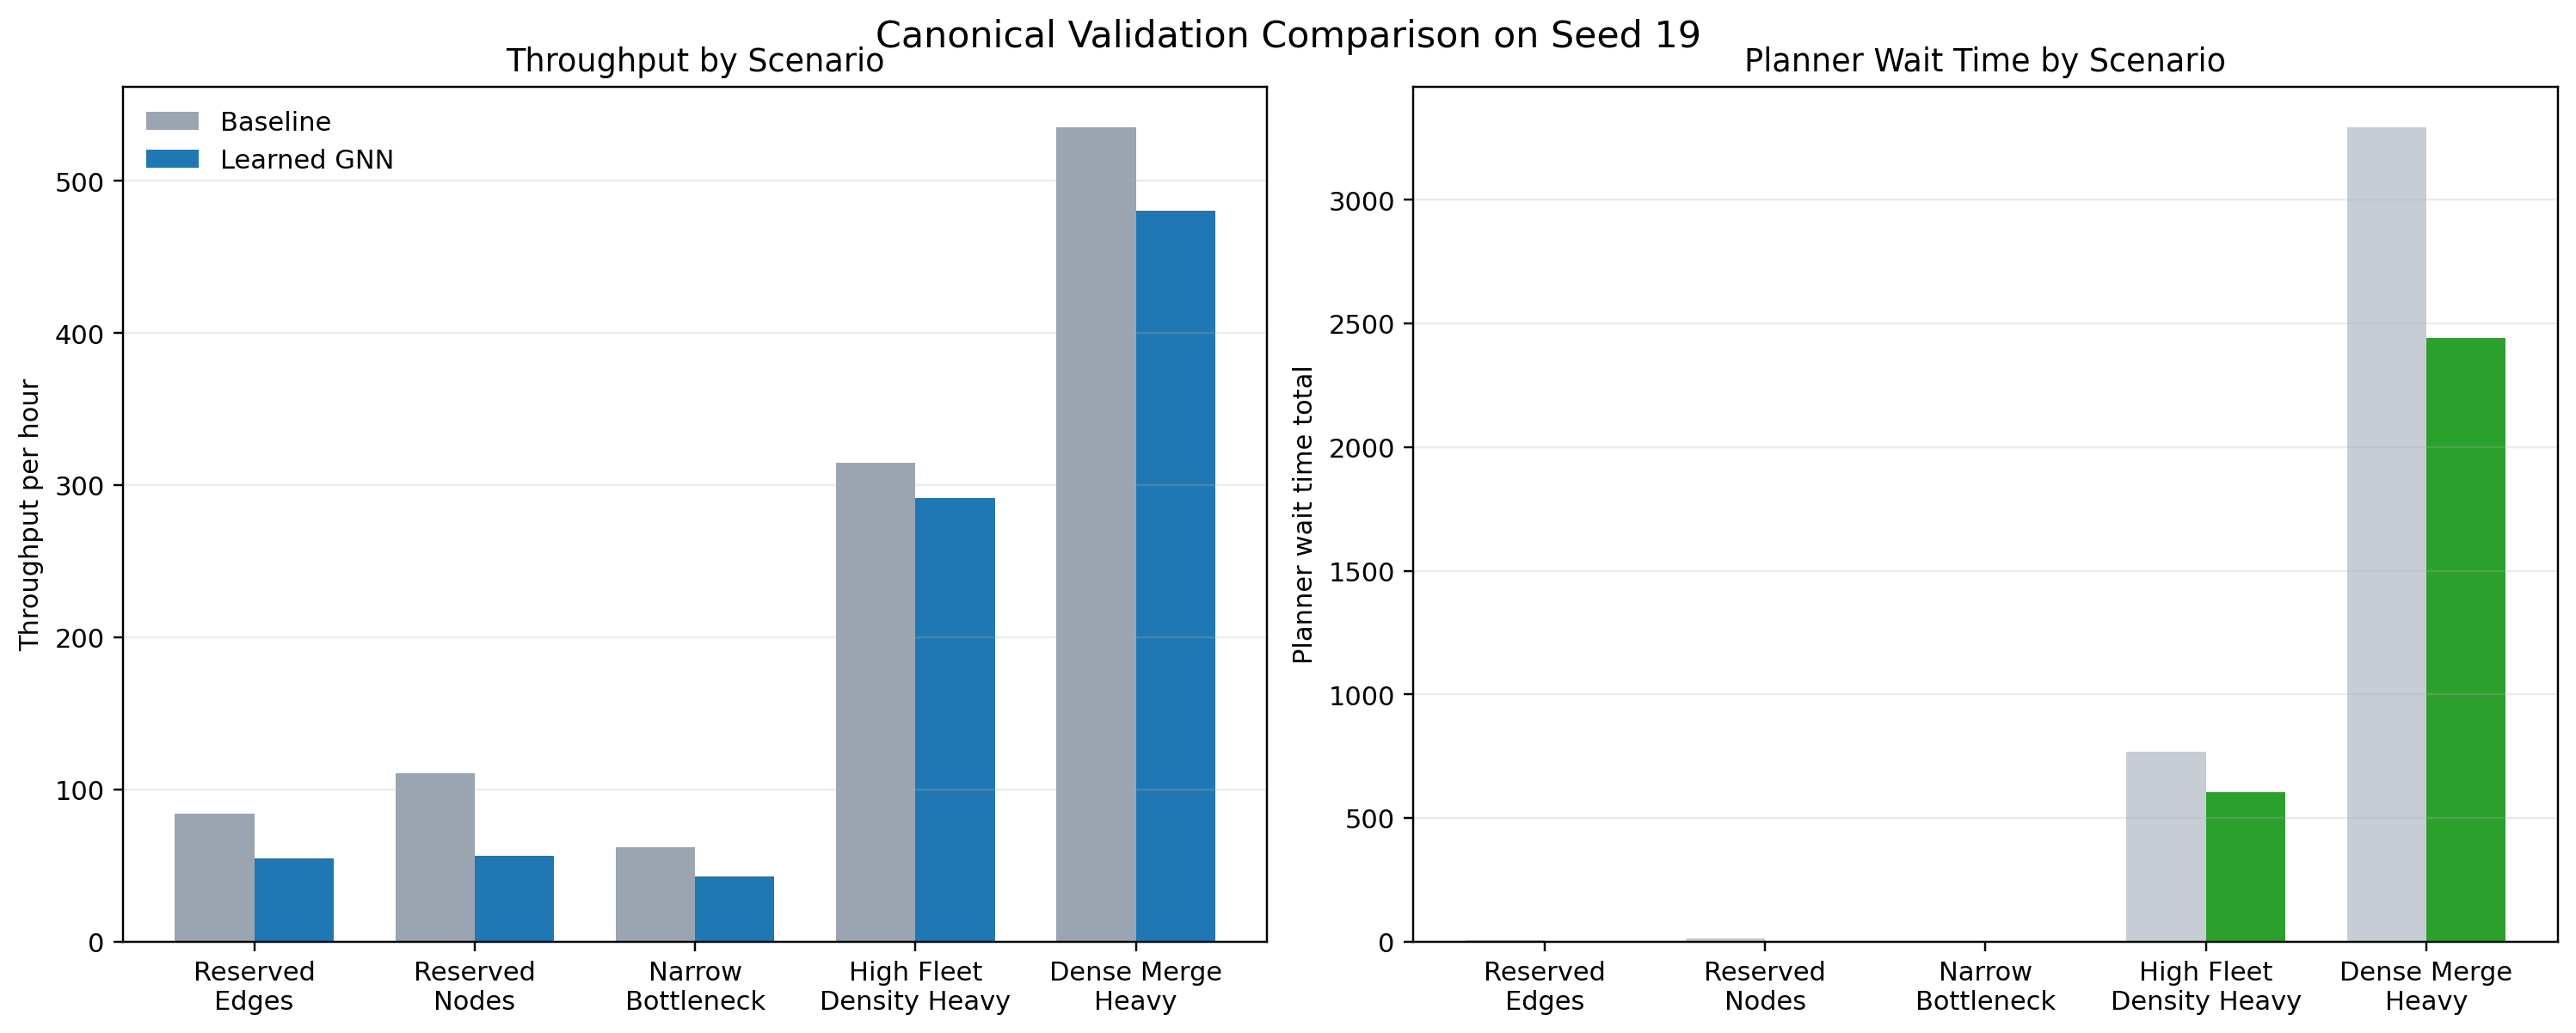
\includegraphics[width=\textwidth]{figures/scenario_comparison.png}
\caption{Raw scenario-level comparison on the canonical validation seed. The learned policy reduces planner wait in the dense heavy settings and remains closest to throughput parity in those same difficult scenarios.}
\label{fig:scenario-comparison}
\end{figure}

\begin{figure}[H]
\centering
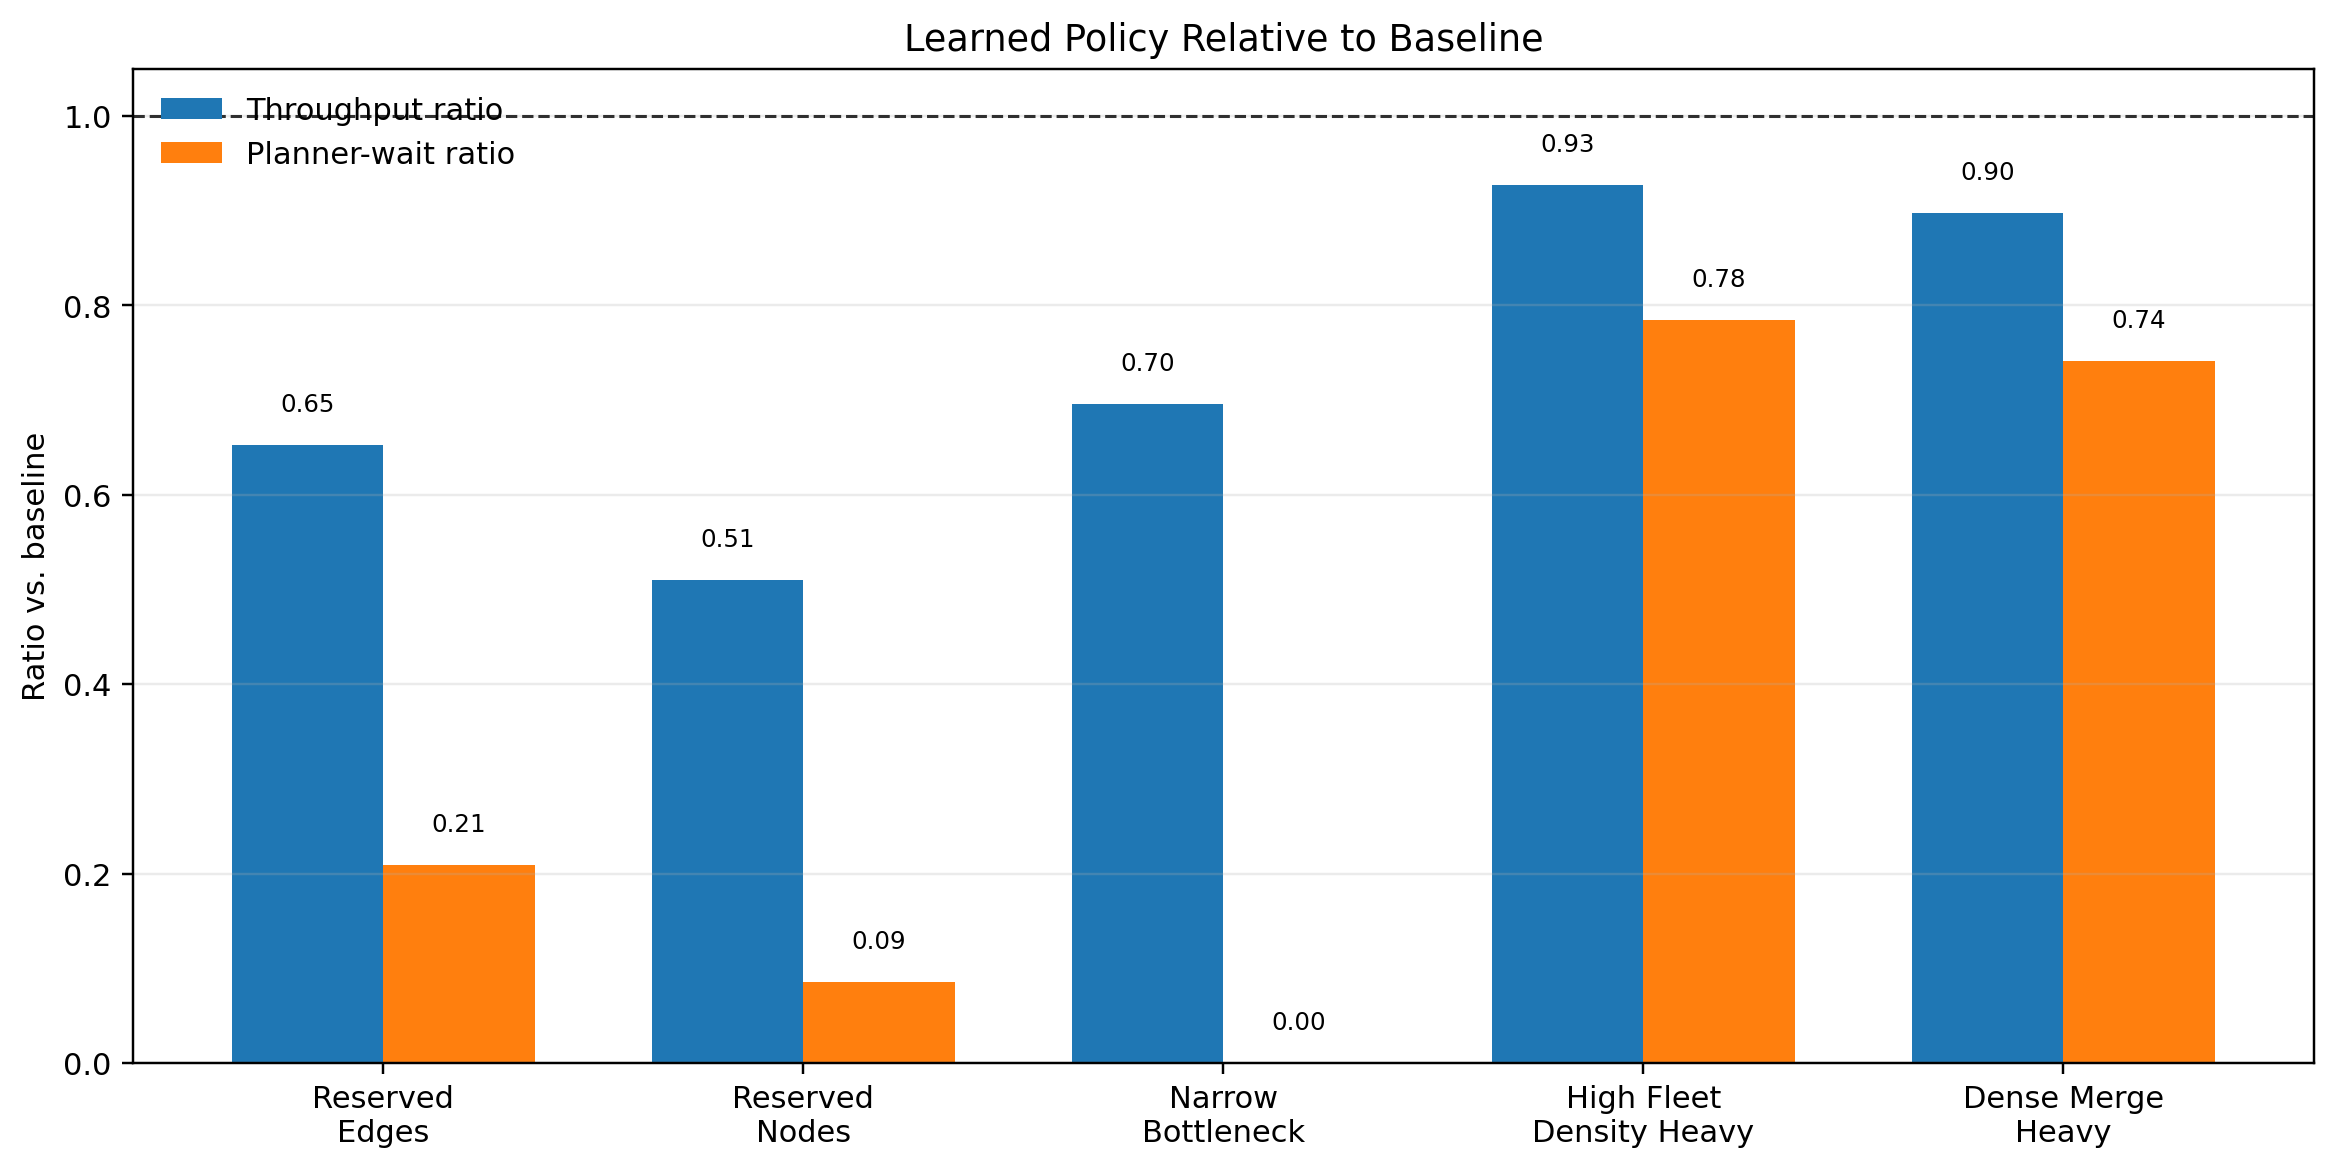
\includegraphics[width=0.9\textwidth]{figures/scenario_ratios.png}
\caption{Relative performance versus the heuristic baseline. The dashed line at 1.0 marks parity. Values below 1.0 are better for planner-wait ratio, but worse for throughput ratio. The learned policy is closest to parity on the dense heavy scenarios and much worse on the easier scenarios.}
\label{fig:scenario-ratios}
\end{figure}

\subsection{Interpretation}
The results are mixed.

\paragraph{Where the learned policy helps.}
On the two dense heavy scenarios, the learned policy reduces planner waiting relative to the baseline:
\begin{itemize}[leftmargin=1.5em]
    \item \texttt{integrated\_high\_fleet\_density\_heavy}: planner wait falls to 78.5\% of baseline.
    \item \texttt{integrated\_dense\_merge\_heavy}: planner wait falls to 74.1\% of baseline.
\end{itemize}

On \texttt{integrated\_dense\_merge\_heavy}, the learned policy also reports zero pre-resolution path conflicts while the baseline reports 764. Even if this metric should be interpreted cautiously, it is directionally consistent with the intended dense-traffic objective.

\paragraph{Where the learned policy still needs improvement.}
The learned policy loses throughput on the easier and medium-difficulty scenarios:
\begin{itemize}[leftmargin=1.5em]
    \item \texttt{reserved\_edges}: 65.3\% of baseline throughput
    \item \texttt{reserved\_nodes}: 51.1\% of baseline throughput
    \item \texttt{narrow\_bottleneck}: 69.6\% of baseline throughput
\end{itemize}

It also remains close to the teacher:
\[
\text{distinctness vs. teacher} = 0.0056 \ll 0.05.
\]

This suggests the final policy did not yet separate enough from imitation during PPO fine-tuning, even though the dense-scenario behavior is already directionally promising.

\begin{figure}[H]
\centering
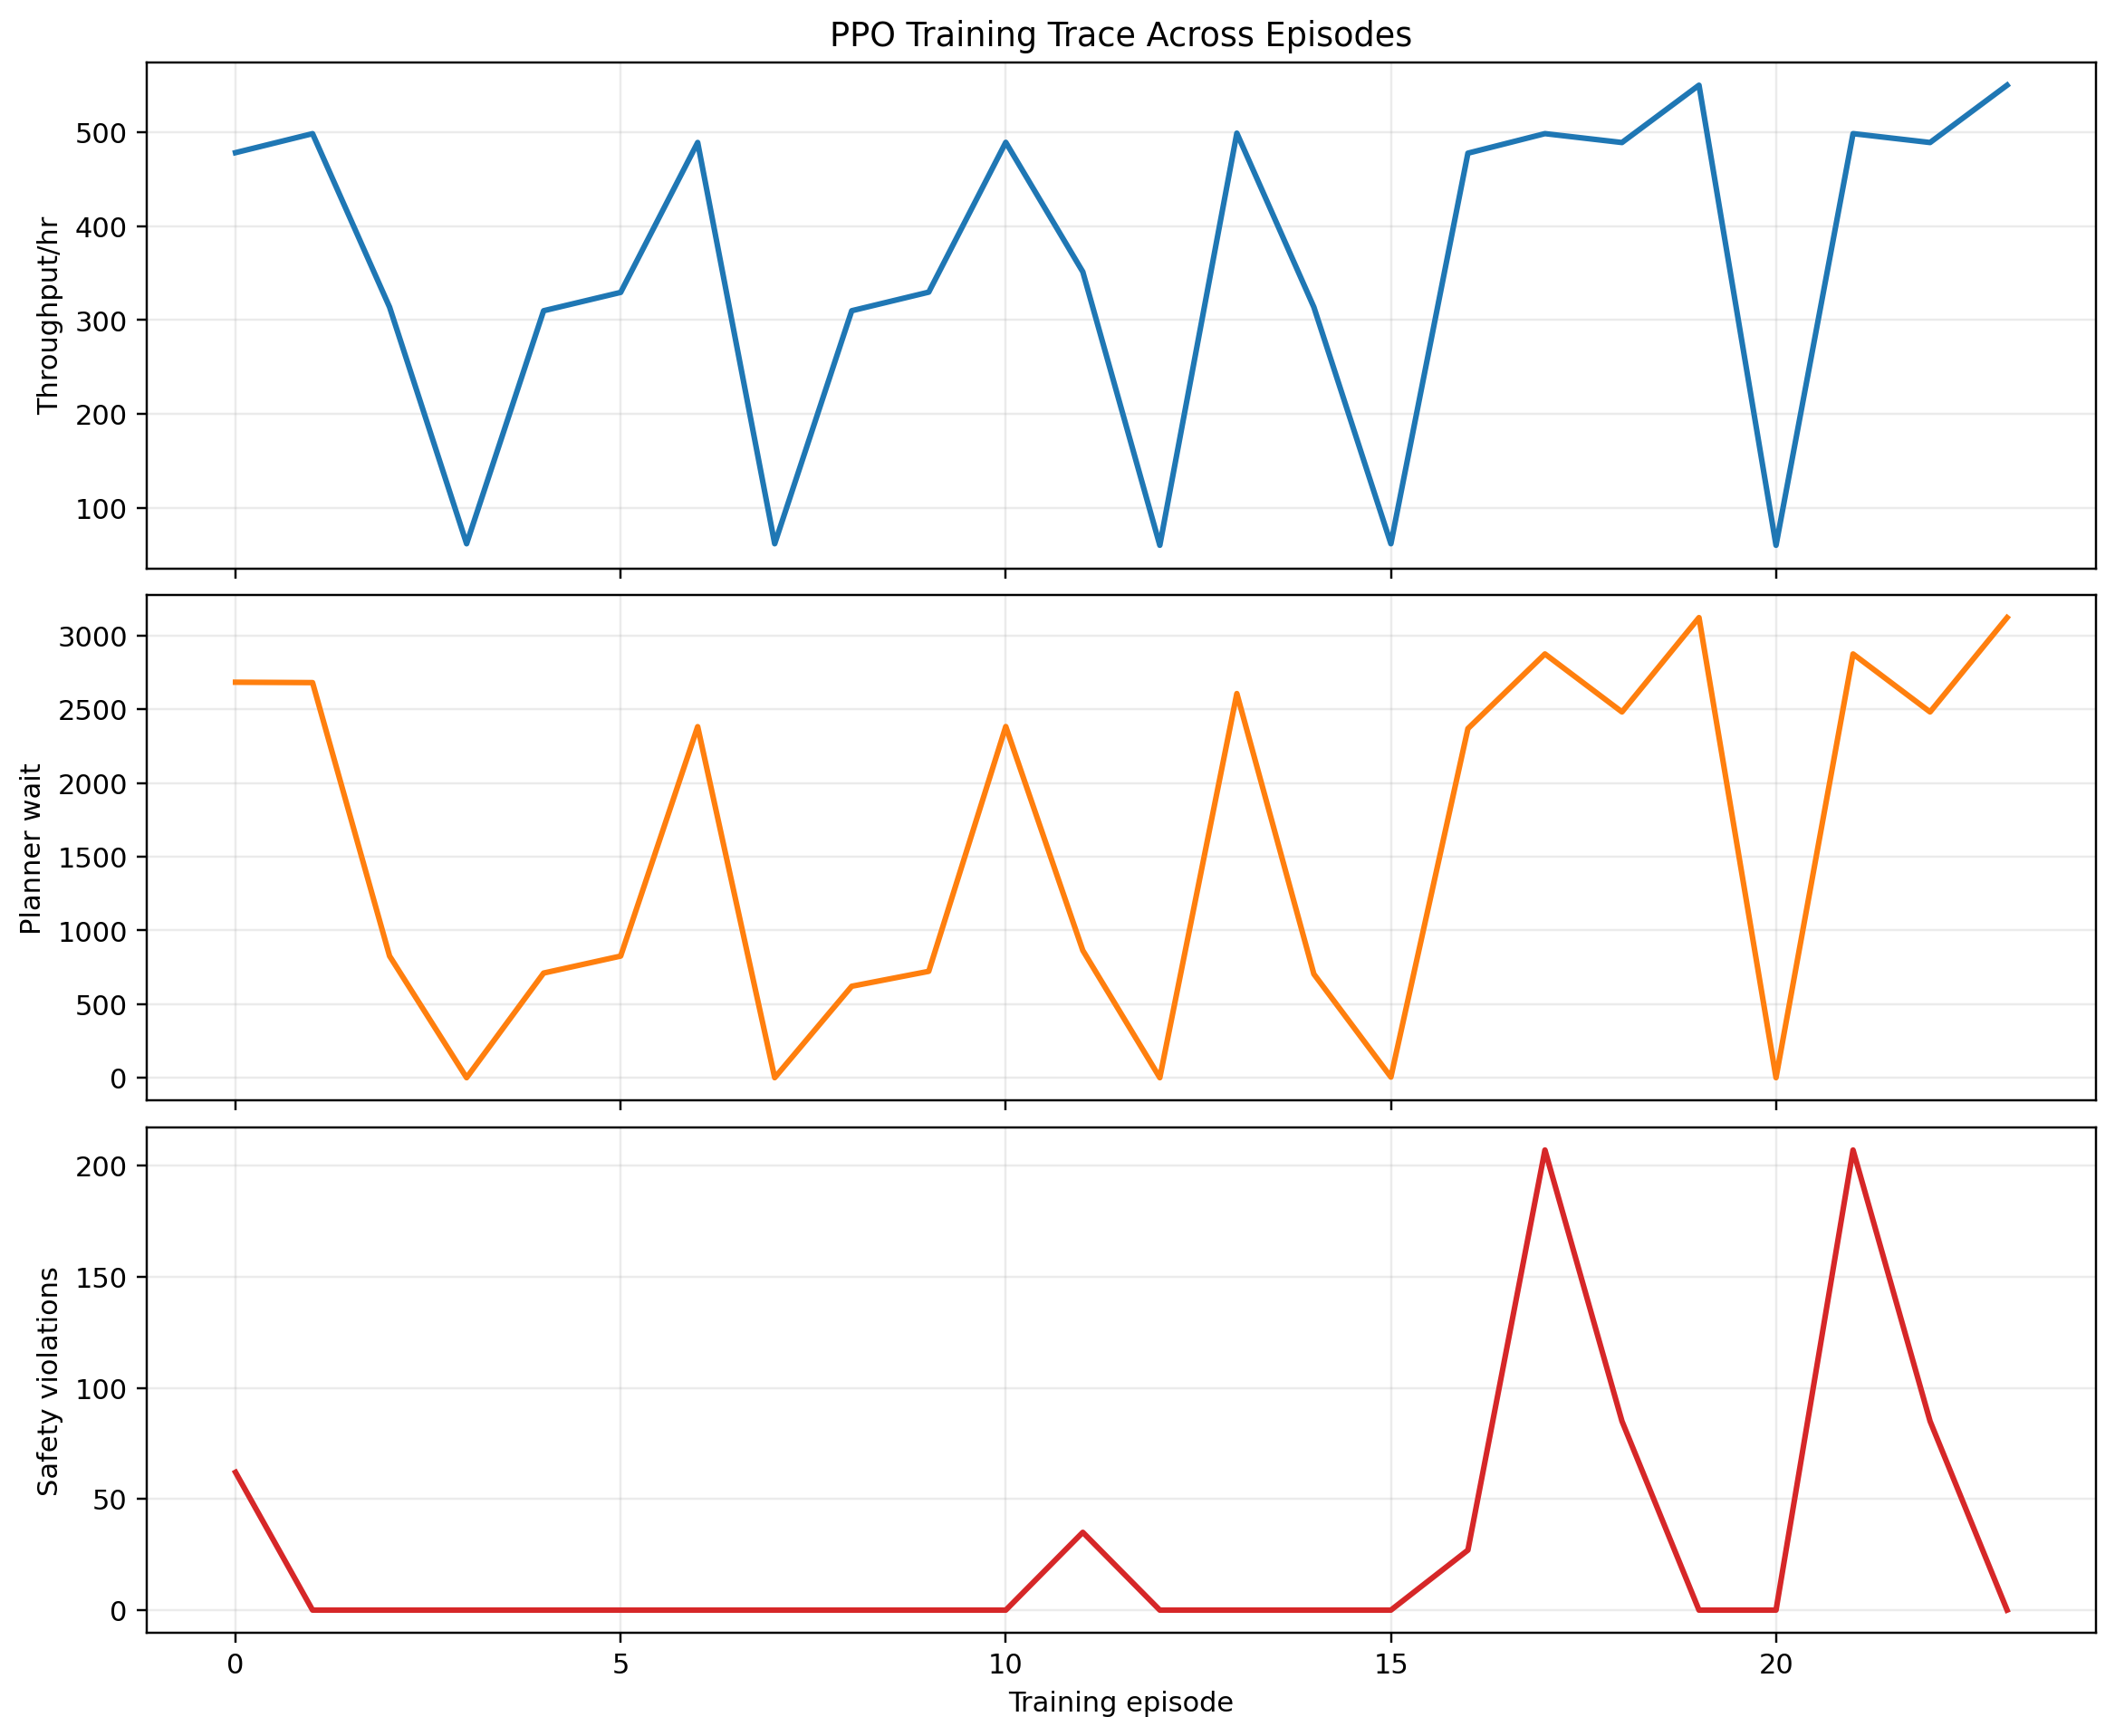
\includegraphics[width=0.92\textwidth]{figures/ppo_training_trace.png}
\caption{PPO training trace over 24 episodes. Dense scenarios dominate the later curriculum, throughput remains high in dense-merge episodes, and the policy repeatedly achieves strong dense-traffic performance. The remaining opportunity is to translate that dense-scenario competence into more uniform performance across the full benchmark suite.}
\label{fig:ppo-trace}
\end{figure}

\section{Discussion}
The original project goal was to demonstrate that a GNN-based policy could beat standard baselines, especially in dense traffic. The current evidence supports an important partial version of that claim.

The strongest conclusion is:
\begin{quote}
The conflict-aware GNN policy is already competitive in the hardest dense-traffic scenarios, where it reduces planner waiting and conflict pressure while maintaining safe operation, and the overall framework provides a strong benchmark foundation for future learning-based improvements.
\end{quote}

This is a meaningful result. It means the representation is learning something relevant to dense interaction structure, and it validates the core design choice of using an integrated conflict-aware graph policy rather than studying dispatch or path planning in isolation.

Figures~\ref{fig:scenario-comparison} and~\ref{fig:scenario-ratios} make the main tradeoff clear: the learned controller is already strong as a congestion-reduction policy and comes closest to baseline throughput precisely in the dense settings that matter most to the project motivation. Figure~\ref{fig:warm-start} explains why the policy remains conservative: behavior cloning drove it extremely close to the teacher before PPO began. Figure~\ref{fig:ppo-trace} then shows that PPO training repeatedly achieves high-performing dense episodes, suggesting that the remaining gap is not whether RL can help, but how to stabilize and generalize those gains across the full benchmark.

\subsection{Benchmark Contribution}
An important outcome of this project is the benchmark itself. The simulator now provides:
\begin{itemize}[leftmargin=1.5em]
    \item a common warehouse graph environment for integrated coordination,
    \item multiple scenarios ranging from easier reserved-lane layouts to dense heavy traffic,
    \item fixed seeds and reproducible artifact generation,
    \item standardized metrics for throughput, safety, congestion, and conflict,
    \item a common evaluation path for heuristic, imitation, and RL-based policies.
\end{itemize}

This matters because future work in ML and RL for warehouse coordination needs common ground. Without a shared simulator, scenario suite, and metrics package, results are hard to compare fairly. This project contributes that shared experimental foundation.

\subsection{Why the RL Results Are Still Positive}
Even though the final aggregate gate is not fully passed, the RL results are still positive in several ways:
\begin{itemize}[leftmargin=1.5em]
    \item the policy remains safe on the canonical validation suite,
    \item it achieves full task completion,
    \item it reduces planner wait in the dense heavy scenarios,
    \item it reaches near-parity throughput in the dense heavy scenarios,
    \item it eliminates a large number of pre-resolution path conflicts in \texttt{integrated\_dense\_merge\_heavy}.
\end{itemize}

Taken together, these results show that RL is not failing outright. Instead, it is already learning useful dense-traffic coordination behavior, and the next stage of work is to improve training stability and better preserve throughput on easier scenarios.

\section{Limitations}
Several limitations affect the strength of the conclusions:
\begin{itemize}[leftmargin=1.5em]
    \item The final canonical evaluation used a single validation seed per scenario, which is too small for strong statistical claims.
    \item The learned policy was heavily shaped by behavior cloning, and the warm-start match rate suggests imitation collapse.
    \item The aggregate claim gate is dominated by throughput losses on simpler scenarios, which may obscure scenario-specific dense-traffic gains.
    \item Some metrics are asymmetric across scenarios. For example, pre-resolution path conflicts are informative in \texttt{dense\_merge\_heavy} but are zero across several other scenarios.
    \item The current report is based on artifact-level summaries and validation outputs; a stronger final study would include multiple seeds, confidence intervals, and explicit ablations.
\end{itemize}

\section{Conclusions}
This project successfully addresses a real warehouse coordination problem with an explicit stochastic simulation and quantitative outputs. The codebase models the right system: graph-structured robot motion, stochastic tasks, integrated coordination decisions, congestion, and safety. It also demonstrates a complete learning pipeline with warm start, PPO training, checkpointing, and benchmark evaluation.

The final empirical conclusion is that the current GNN policy is \emph{promising and already useful in dense traffic}, even though it is not yet uniformly superior on every benchmark metric. It preserves safety, helps on dense-traffic waiting and conflict metrics, and demonstrates that integrated graph-based RL is a credible direction for warehouse coordination.

Just as importantly, the project delivers a well-defined simulation and benchmarking framework that future ML and RL methods can build on. That infrastructure contribution is significant on its own because it turns a difficult coordination problem into a reproducible experimental platform.

Future work should focus on:
\begin{enumerate}[leftmargin=1.5em]
    \item reducing teacher collapse during warm start,
    \item increasing PPO pressure on throughput recovery,
    \item evaluating with multiple seeds and confidence intervals,
    \item tuning dense-only objectives separately from easy-scenario generalization.
\end{enumerate}

\section{Reproducibility}
The main training run used the following command:
\begin{verbatim}
PYTHONPATH=src python3 -m warehouse_sim.learning.cli train-integrated-rl \
  --config configs/canonical_artifacts/canonical_macro_ppo_training.toml
\end{verbatim}

Key implementation characteristics of the final pipeline include:
\begin{itemize}[leftmargin=1.5em]
    \item CPU worker parallelism for rollout and warm-start trace collection,
    \item MPS learner execution on Apple Silicon,
    \item checkpointing and resume support,
    \item minibatched behavior cloning and PPO updates,
    \item fixed seeds in the canonical curriculum and validation configuration.
\end{itemize}

\section*{Appendix: Key Output Files}
The main outputs used in this report were:
\begin{itemize}[leftmargin=1.5em]
    \item \texttt{outputs/canonical\_artifacts/macro\_ppo/claim\_gate.json}
    \item \texttt{outputs/canonical\_artifacts/macro\_ppo/evaluation\_rollouts.json}
    \item \texttt{outputs/canonical\_artifacts/macro\_ppo/training\_metrics.csv}
    \item \texttt{outputs/canonical\_artifacts/macro\_ppo/warm\_start\_metrics.csv}
    \item \texttt{outputs/canonical\_artifacts/macro\_ppo/baseline\_eval/*/seed\_19/summary.json}
\end{itemize}

\end{document}
